\section{Methodology}
For our dynamic instrumentation we used frida instrumentation tool\cite{frida}. Frida is dynamic instrumentation toolkit which enables inject javascript snippets to applications of all platforms.


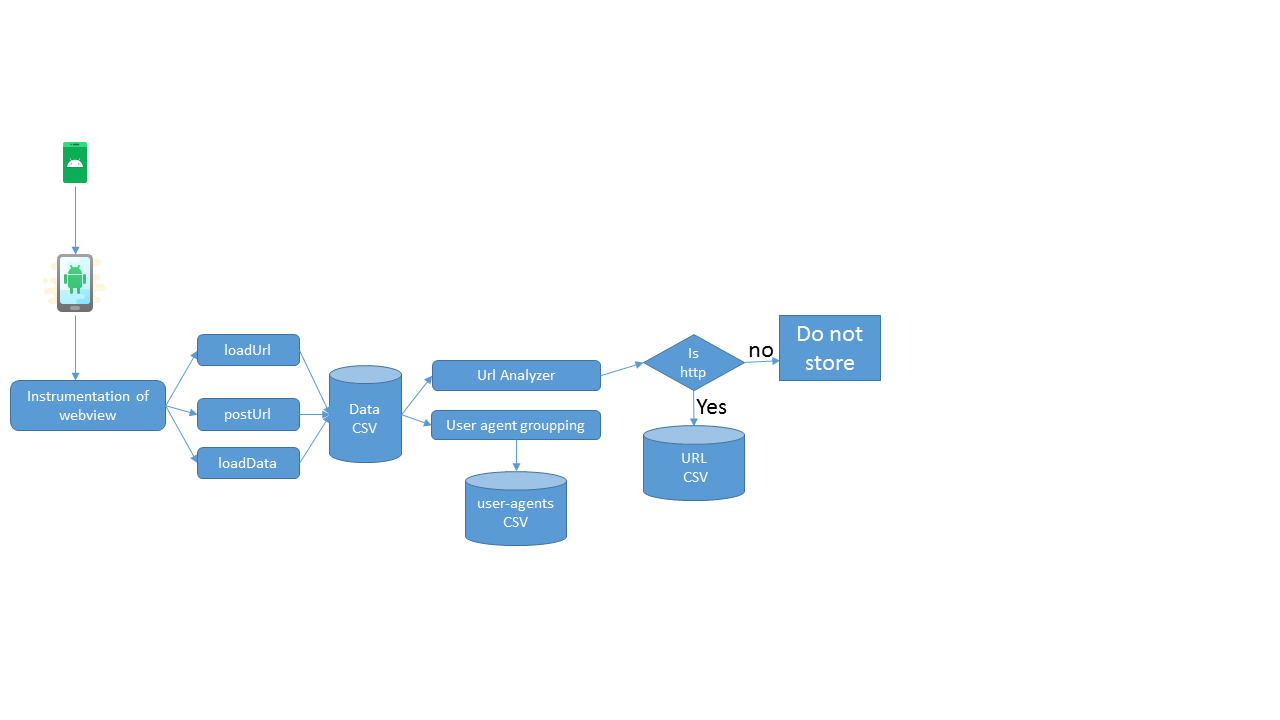
\includegraphics[width=\textwidth]{images/Proccess.PNG}
For instrument our android apps we have implemented the steps below:\\
1. Download frida server from release page.\\
2. Copy downloaded file into device or emulator.\\ 
3. Run the server inside the device.\\
After above steps frida server on our device is running. Then in the first step we wrote javascript code to inject to the android application and log webview loadUrl and OnloadResource functions. From this methods we log url, custom header and user-agent strings.\\
\begin{lstlisting}[language=JavaScript, caption=Instrumentation of Webview]    
    'use strict';

if (Java.available) {
    Java.perform(function() {
        //android package name 
        const ActivityThread = Java.use('android.app.ActivityThread');
        var context = ActivityThread.currentApplication().getApplicationContext();
        var packagename = context.getPackageName();
        
        var WebView = Java.use("android.webkit.WebView");
        //Instrumenting webview.loadUrl 
        WebView.loadUrl.overload('java.lang.String').implementation = function(url) {
            this.loadUrl(url);
            //Sending to python code record logs
            send({
                packageName: packagename,
                method: "loadUrl",
                Url: url,
                Header: "",
                userAgent: this.getSettings().getUserAgentString()
            });
        }
           //Instrumenting webview.loadUrl with custom headers
        WebView.loadUrl.overload('java.lang.String', 'java.util.Map').implementation = function(url, header) {
            this.loadUrl(url, header);
               //Unmapping custom headers
            var keyset = p1.keySet();
            var it = keyset.iterator();
            while (it.hasNext()) {
                var keystr = it.next().toString();
                var valuestr = p1.get(keystr).toString();
            }
         //Sending to python code record logs
            send({
                method: "loadUrlHeader",
                Url: url,
                Header: header,
                userAgent: this.getSettings().getUserAgentString()
            });
        }
        var WebViewClient = Java.use("android.webkit.WebViewClient");
          //Instrumenting webviewclient.onLoadResource
        WebViewClient.onLoadResource.overload('android.webkit.WebView', 'java.lang.String').implementation = function(webview, url) {
            send({
                packageName: packagename,
                method: "onLoadResource",
                Header: "",
                Url: url,
                userAgent: webview.getSettings().getUserAgentString()
            });
            this.onLoadResource(webview, url);
        }
    });

}
      \end{lstlisting}    

Second step is for automatization of injection proccess in the python scripts.In Listing 2 you can see our code:\\
\begin{lstlisting}[language=Python, caption=Installation] 
import time

from ppadb.client import Client as AdbClient
import re
import os
import csv
import frida
path = 'path/to/the/applications/folder'
path1='path/to/the/tested/applications/folder'

#Connects to device
def connect():
  
    client = AdbClient(host="127.0.0.1", port=5037) 
    devices = client.devices()
    if len(devices) == 0:
        print('No devices')
        quit()
    device = devices[0]
    print(f'Connected to {device}')
    return device, client

def search_package_in_avd(device):
    command = device.shell('pm list packages -3 '+'|cut -f 2 -d '+':')
    packages=re.split(':|\r|\n',command)
    for package in packages:
     print(package+"\n")
    if not packages:
        return ""
    else:
        return packages
#Reads apk file names in folder        
def read_files():
    files = os.listdir(path)
    return files

def install_package(package):
    try:
     device.install(path+'/'+package)
     print(package+" installed ")
     return True
    except Exception as e:
     print("Error"+str(e))
     os.remove(path+"/"+package)
     return False
    
def uninstall_package(device):
     packages=search_package_in_avd(device)
     for package in packages:
        device.uninstall(package)
        print(package+" uninstalled")
#Initialize csv file writing
def file_init():
    header = ["packageName","package","method","header","url","user agent"]
    file = open('user_agents.csv', 'a')
    writer = csv.writer(file)
    writer.writerow(header)    
    return file,writer
#Write into csv file
def file_open1():
    file = open('user_agents.csv', 'a')
    writer = csv.writer(file)
    return file,writer    
def add_rows(writer,data):
    writer.writerow(data)
#frida instrumentation
def frida_instument():
  try:
    device_frida = frida.get_usb_device()
    f_package=search_package_in_avd(device)[0];
    pid = device_frida.spawn([f_package])
    session = device_frida.attach(pid)
    script = session.create_script(open("instrumentJs.js").read())
    script.on("message", on_message)
    script.load()
    device_frida.resume(pid)
    time.sleep(5)
  except Exception as e:
    print("ERROR"+" "+str(e))
#Listens messages from injected js code and records to file  
def on_message(message, data):
    print("frida")
    if 'payload' in message:
        payload = message['payload']  
        if 'Url' in payload:
            print("inFrida")
            data=[payload['packageName'],package,payload['method'],payload['Header'],payload['Url'], payload['userAgent']]
            file,writer=file_open1() 
            add_rows(writer,data)
            file.close()
            
device=None
writer=None
file=None
package=None
f_package=None
if __name__ == '__main__':
    file,writer=file_init() 
    device, client = connect()     
    uninstall_package(device)
    apks=read_files() 
    for apk in apks:
       x=install_package(apk)
       package=apk
       if(x):
        frida_instument()
        uninstall_package(device)
        os.replace(path+"/"+apk,path1+"/"+apk)       
    file.close()
    \end{lstlisting}   




Above code implements below functions:\\
1. Application installation and removal \\
2. Instruments the webview to Log information .\\

Third step is processing obtained data:
\begin{lstlisting}[language=Python, caption=Proccessing the obtained data] 
import os
import csv
url={}
useragent={}

with open('user_agents.csv', newline='') as csvfile:
        reader = csv.DictReader(csvfile)
        for row in reader:
         #Grouped unencrypted traffic by packages       
         if row["packageName"] not in url:
          if "http://" in row["url"]:
           url[row["packageName"]]=[]
           url[row["packageName"]].append(row["url"])
         elif "http://" in row["url"] :
          url[row["packageName"]].append(row["url"])
         #Grouped user agents by  packages  
         if  row["user agent"] not in useragent:
           useragent[row["user agent"]]=[]
           useragent[row["user agent"]].append(row["packageName"])
         else:
           useragent[row["user agent"]].append(row["packageName"])       
      
  
       
       
        file = open('url.csv', 'a')
        writer = csv.writer(file)  
        header = ["packageName","url"] 
        writer.writerow(header)        
        for key, value in url.items():
            data=[key,value]
            writer.writerow(data)
                
                
        file = open('useragents1.csv', 'a')
        writer = csv.writer(file)  
        header = ["useragents","package"]
        writer.writerow(header)   
        for key, value in useragent.items():
            data=[key,"|",value]
            writer.writerow(data)       

   \end{lstlisting}  
       

 The data collection was done in an emulator. In this emulator, I signed up with a dummy email address on google. This is how I know if an app is using my google ads id, my GSF id, or some personal settings.  
 We used the adb package to install apps on the emulator. 



After collecting all the data we created a simple python program to analyze the data. 
1. Grouping user agent rows.
User agent grouping.  To review the different user agents. 
2. Find unencrypted traffic. 
Find unencrypted traffic and match it with a packet. We have separated the unencrypted packet that sends sensitive information and that is not malicious.
